\subsubsection{Phase 4: Erstellen von Verbindungen zwischen den Seiten}

Wenn auf einen Link geklickt oder einfach ein Formular bestätigt wird,
wird man normalerweise auf eine andere Seite weitergeleitet. Diese Phase
befasst sich im Wesentlichen mit der Umsetzung dieser Aufgabe.
Im Rahmen der Implementierung des Registrierungstests geht es darum,
die Seiten zwischen zwei Aktionen miteinander zu verbinden.
Zum Beispiel sollte die Registrierungsfunktion nach einem Klick
auf den Button Login die RegisterPage zurückgeben (siehe \Cref{fig:reg-page}).
Dies ist in der Tat eine Modellierung der Web-Navigation in Java.
Diese Arbeit muss durchgeführt werden und macht in der letzten Phase
Sinn.

\begin{figure}[H]
    \centering
    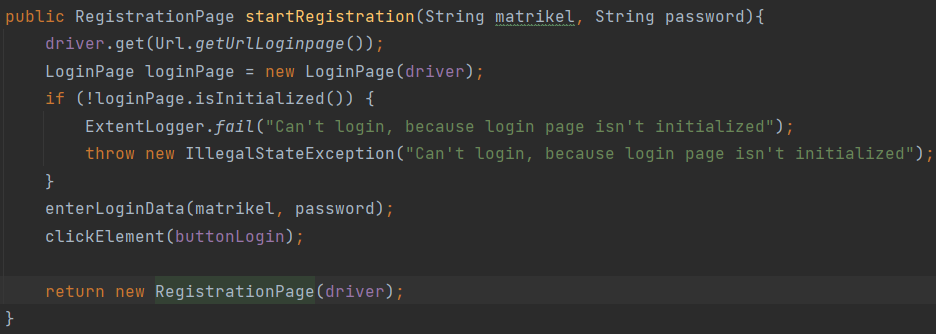
\includegraphics[scale=0.5]{images/reg-page}
    \caption{StartRegistration Funktion} \label{fig:reg-page}
\end{figure}
